%%
%% Copyright 2007-2018 Elsevier Ltd
%%
%% This file is part of the 'Elsarticle Bundle'.
%% ---------------------------------------------
%%
%% It may be distributed under the conditions of the LaTeX Project Public
%% License, either version 1.2 of this license or (at your option) any
%% later version.  The latest version of this license is in
%%    http://www.latex-project.org/lppl.txt
%% and version 1.2 or later is part of all distributions of LaTeX
%% version 1999/12/01 or later.
%%
%% The list of all files belonging to the 'Elsarticle Bundle' is
%% given in the file `manifest.txt'.
%%

%% Template article for Elsevier's document class `elsarticle'
%% with numbered style bibliographic references
%% SP 2008/03/01
%%
%%
%%
%% $Id: elsarticle-template-num.tex 64 2013-05-15 12:23:51Z rishi $
%%
%%
\documentclass{article}

%% Use the option review to obtain double line spacing
%\documentclass[authoryear,preprint,review,12pt]{elsarticle}

%% Use the options 1p,twocolumn; 3p; 3p,twocolumn; 5p; or 5p,twocolumn
%% for a journal layout:
%\documentclass[final,1p,times]{elsarticle}
%\documentclass[final,1p,times,twocolumn]{elsarticle}
%\documentclass[final,3p,times]{elsarticle}
%\documentclass[final,3p,times,twocolumn]{elsarticle}
%\documentclass[final,5p,times]{elsarticle}
%\documentclass[final,5p,times,twocolumn]{elsarticle}

%% For including figures, graphicx.sty has been loaded in
%% elsarticle.cls. If you prefer to use the old commands
%% please give \usepackage{epsfig}

%% The amssymb package provides various useful mathematical symbols
\usepackage{amssymb}
\usepackage{amsmath}

%% The amsthm package provides extended theorem environments
\usepackage{amsthm}
\usepackage{algorithm}
\usepackage{algorithmic}

\renewcommand{\algorithmicrequire}{\textbf{Input:}}
\renewcommand{\algorithmicensure}{\textbf{Output:}}


\usepackage{subcaption}
\usepackage{tikz}
\usetikzlibrary{arrows,decorations.markings}
\usetikzlibrary{intersections, calc}

%% The lineno packages adds line numbers. Start line numbering with
%% \begin{linenumbers}, end it with \end{linenumbers}. Or switch it on
%% for the whole article with \linenumbers.
%% \usepackage{lineno}

\begin{document}

\begin{align}
\begin{pmatrix}
1 & 7 & 3 & 1/7\\
1/7 & 1 & 1 & 1/9\\
1/3 & 1 & 1 & 1/9\\
7 & 9 & 9 & 1
\end{pmatrix}
\end{align}
\hspace{\fill}CI=0.093

\noindent
%
\parbox{.45\linewidth}{
    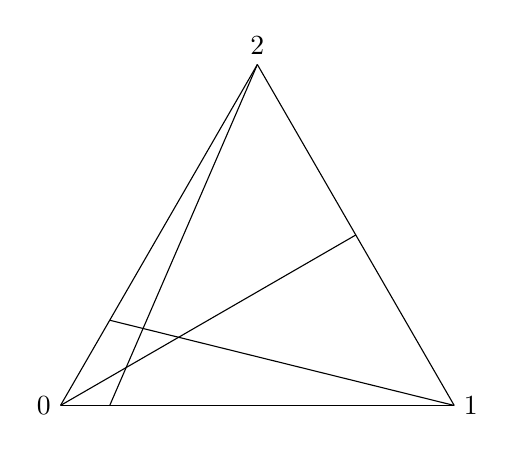
\begin{tikzpicture}[line cap=miter,line join=miter,>=triangle 45]
        %\begin{tikzpicture}[node distance=2.5cm, line cap=miter,line join=miter,>=triangle 45,x=1.0cm,y=1.0cm]
        \def\a{7};
        \def\b{1};
        \def\c{1/3};
        \def\scale{2.5};

        \coordinate (x) at (0,0);% node at (x) [left]{$\boldsymbol{X}$};
        \coordinate (y) at (2*\scale,0);%
        \coordinate (z) at (1*\scale, 1.7320508*\scale);%
        \draw [name path=xy] (x) -- (y);  \draw [name path=yz] (y) -- (z); \draw [name path=zx] (z) -- (x);
        \node at (x) [left] {$0$}; \node at (y) [right]{$1$}; \node at (z) [above]{$2$};

        \coordinate (s) at ($(x)!1/(1+\a)!(y)$);    \coordinate (t) at ($(y)!1/(1+\b)!(z)$);    \coordinate (u) at ($(z)!1/(1+\c)!(x)$);
        %\node at (s) [below] {$\boldsymbol{S}$}; \node at (t) [right]{$\boldsymbol{T}$}; \node at (u) [left]{$\boldsymbol{U}$};

        \draw [name path=zs] (z) -- (s);
        \draw [name path=xt] (x) -- (t);
        \draw [name path=yu] (y) -- (u);

        %\fill[name intersections={of=zs and yu}]   (intersection-1) circle (0pt) node [above right] {$\boldsymbol{A}$};
        %\fill[name intersections={of=zs and xt}]   (intersection-1) circle (0pt) node [above left] {$\boldsymbol{B}$};
        %\fill[name intersections={of=yu and xt}]   (intersection-1) circle (0pt) node [below] {$\boldsymbol{C}$};

        %\coordinate (w) at (1*\scale, 0.55*\scale);
        %\fill (w) circle (2pt) node [above]{$\boldsymbol{w}$};

        %\node at ($(x)!.5!(s)$) [below] {$1$}; \node at ($(s)!.5!(y)$) [below] {$a_{12}$};
        %\node at ($(y)!.5!(t)$) [right] {$1$}; \node at ($(t)!.5!(z)$) [right] {$a_{23}$};
        %\node at ($(z)!.5!(u)$) [left] {$1$}; \node at ($(u)!.5!(x)$) [left] {$a_{31}$};
    \end{tikzpicture}
    \\
    Pairwise comparison values $012$.
}
~~~~
\parbox{.45\linewidth}{
    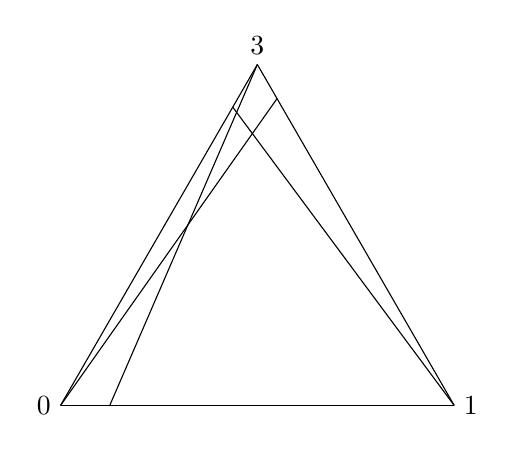
\begin{tikzpicture}[line cap=miter,line join=miter,>=triangle 45]
        %\begin{tikzpicture}[node distance=2.5cm, line cap=miter,line join=miter,>=triangle 45,x=1.0cm,y=1.0cm]
        \def\a{7};
        \def\b{1/9};
        \def\c{7};
        \def\scale{2.5};

        \coordinate (x) at (0,0);% node at (x) [left]{$\boldsymbol{X}$};
        \coordinate (y) at (2*\scale,0);%
        \coordinate (z) at (1*\scale, 1.7320508*\scale);%
        \draw [name path=xy] (x) -- (y);  \draw [name path=yz] (y) -- (z); \draw [name path=zx] (z) -- (x);
        \node at (x) [left] {$0$}; \node at (y) [right]{$1$}; \node at (z) [above]{$3$};

        \coordinate (s) at ($(x)!1/(1+\a)!(y)$);    \coordinate (t) at ($(y)!1/(1+\b)!(z)$);    \coordinate (u) at ($(z)!1/(1+\c)!(x)$);
        %\node at (s) [below] {$\boldsymbol{S}$}; \node at (t) [right]{$\boldsymbol{T}$}; \node at (u) [left]{$\boldsymbol{U}$};

        \draw [name path=zs] (z) -- (s);
        \draw [name path=xt] (x) -- (t);
        \draw [name path=yu] (y) -- (u);

        %\fill[name intersections={of=zs and yu}]   (intersection-1) circle (0pt) node [above right] {$\boldsymbol{A}$};
        %\fill[name intersections={of=zs and xt}]   (intersection-1) circle (0pt) node [above left] {$\boldsymbol{B}$};
        %\fill[name intersections={of=yu and xt}]   (intersection-1) circle (0pt) node [below] {$\boldsymbol{C}$};

        %\coordinate (w) at (1*\scale, 0.55*\scale);
        %\fill (w) circle (2pt) node [above]{$\boldsymbol{w}$};

        %\node at ($(x)!.5!(s)$) [below] {$1$}; \node at ($(s)!.5!(y)$) [below] {$a_{12}$};
        %\node at ($(y)!.5!(t)$) [right] {$1$}; \node at ($(t)!.5!(z)$) [right] {$a_{23}$};
        %\node at ($(z)!.5!(u)$) [left] {$1$}; \node at ($(u)!.5!(x)$) [left] {$a_{31}$};
    \end{tikzpicture}
    \\
Pairwise comparison values $013$.
}

~~

\noindent
\parbox{.45\linewidth}{
    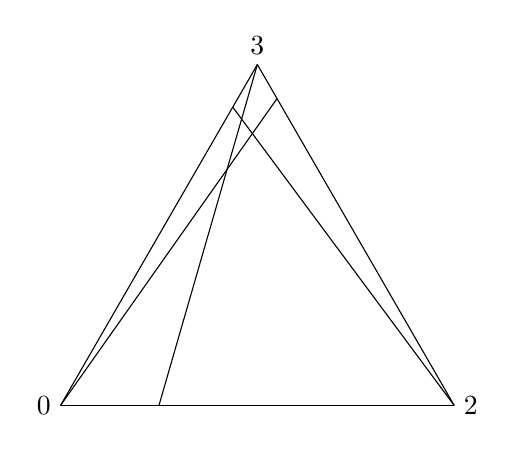
\begin{tikzpicture}[line cap=miter,line join=miter,>=triangle 45]
        %\begin{tikzpicture}[node distance=2.5cm, line cap=miter,line join=miter,>=triangle 45,x=1.0cm,y=1.0cm]
        \def\a{3};
        \def\b{1/9};
        \def\c{7};
        \def\scale{2.5};

        \coordinate (x) at (0,0);% node at (x) [left]{$\boldsymbol{X}$};
        \coordinate (y) at (2*\scale,0);%
        \coordinate (z) at (1*\scale, 1.7320508*\scale);%
        \draw [name path=xy] (x) -- (y);  \draw [name path=yz] (y) -- (z); \draw [name path=zx] (z) -- (x);
        \node at (x) [left] {$0$}; \node at (y) [right]{$2$}; \node at (z) [above]{$3$};

        \coordinate (s) at ($(x)!1/(1+\a)!(y)$);    \coordinate (t) at ($(y)!1/(1+\b)!(z)$);    \coordinate (u) at ($(z)!1/(1+\c)!(x)$);
        %\node at (s) [below] {$\boldsymbol{S}$}; \node at (t) [right]{$\boldsymbol{T}$}; \node at (u) [left]{$\boldsymbol{U}$};

        \draw [name path=zs] (z) -- (s);
        \draw [name path=xt] (x) -- (t);
        \draw [name path=yu] (y) -- (u);

        %\fill[name intersections={of=zs and yu}]   (intersection-1) circle (0pt) node [above right] {$\boldsymbol{A}$};
        %\fill[name intersections={of=zs and xt}]   (intersection-1) circle (0pt) node [above left] {$\boldsymbol{B}$};
        %\fill[name intersections={of=yu and xt}]   (intersection-1) circle (0pt) node [below] {$\boldsymbol{C}$};

        %\coordinate (w) at (1*\scale, 0.55*\scale);
        %\fill (w) circle (2pt) node [above]{$\boldsymbol{w}$};

        %\node at ($(x)!.5!(s)$) [below] {$1$}; \node at ($(s)!.5!(y)$) [below] {$a_{12}$};
        %\node at ($(y)!.5!(t)$) [right] {$1$}; \node at ($(t)!.5!(z)$) [right] {$a_{23}$};
        %\node at ($(z)!.5!(u)$) [left] {$1$}; \node at ($(u)!.5!(x)$) [left] {$a_{31}$};
    \end{tikzpicture}
    \\
Pairwise comparison values $023$.
}
~~~~
\parbox{.45\linewidth}{
    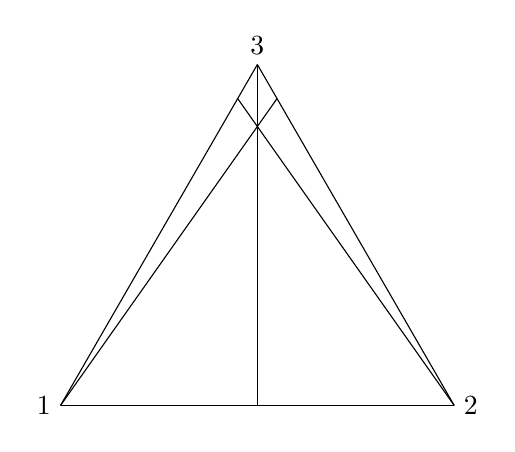
\begin{tikzpicture}[line cap=miter,line join=miter,>=triangle 45]
        %\begin{tikzpicture}[node distance=2.5cm, line cap=miter,line join=miter,>=triangle 45,x=1.0cm,y=1.0cm]
        \def\a{1};
        \def\b{1/9};
        \def\c{9};
        \def\scale{2.5};

        \coordinate (x) at (0,0);% node at (x) [left]{$\boldsymbol{X}$};
        \coordinate (y) at (2*\scale,0);%
        \coordinate (z) at (1*\scale, 1.7320508*\scale);%
        \draw [name path=xy] (x) -- (y);  \draw [name path=yz] (y) -- (z); \draw [name path=zx] (z) -- (x);
        \node at (x) [left] {$1$}; \node at (y) [right]{$2$}; \node at (z) [above]{$3$};

        \coordinate (s) at ($(x)!1/(1+\a)!(y)$);    \coordinate (t) at ($(y)!1/(1+\b)!(z)$);    \coordinate (u) at ($(z)!1/(1+\c)!(x)$);
        %\node at (s) [below] {$\boldsymbol{S}$}; \node at (t) [right]{$\boldsymbol{T}$}; \node at (u) [left]{$\boldsymbol{U}$};

        \draw [name path=zs] (z) -- (s);
        \draw [name path=xt] (x) -- (t);
        \draw [name path=yu] (y) -- (u);

        %\fill[name intersections={of=zs and yu}]   (intersection-1) circle (0pt) node [above right] {$\boldsymbol{A}$};
        %\fill[name intersections={of=zs and xt}]   (intersection-1) circle (0pt) node [above left] {$\boldsymbol{B}$};
        %\fill[name intersections={of=yu and xt}]   (intersection-1) circle (0pt) node [below] {$\boldsymbol{C}$};

        %\coordinate (w) at (1*\scale, 0.55*\scale);
        %\fill (w) circle (2pt) node [above]{$\boldsymbol{w}$};

        %\node at ($(x)!.5!(s)$) [below] {$1$}; \node at ($(s)!.5!(y)$) [below] {$a_{12}$};
        %\node at ($(y)!.5!(t)$) [right] {$1$}; \node at ($(t)!.5!(z)$) [right] {$a_{23}$};
        %\node at ($(z)!.5!(u)$) [left] {$1$}; \node at ($(u)!.5!(x)$) [left] {$a_{31}$};
    \end{tikzpicture}
    \\
Pairwise comparison values $123$.
}

\end{document}
%
%